\documentclass[14pt, a4paper]{extarticle}


%%%%%%%%%%%% Пакеты %%%%%%%%%%%%%%%%%%
\usepackage{polyglossia} % языковой пакет

\usepackage{pdfpages} % пакет для импорта pdf-файлов

\usepackage{tocvsec2} %%%%%%%%%%%%%%%%%%%%%%%%%%%%%%%%%

\usepackage{longtable,booktabs,array}

\usepackage{calc}

\usepackage{ulem}

\usepackage{setspace}

\usepackage[labelsep=period]{caption}

\usepackage{caption}

\usepackage{graphicx} % пакет для использования графики (чтобы вставлять рисунки, фотографии и пр.)


% качественные листинги кода
\usepackage{minted}
\usepackage{listings}
\usepackage{lstfiracode}



\usepackage{amsmath} % поддержка математических символов

\usepackage{url} % поддержка url-ссылок

\usepackage{natbib} % менеджер цитирования natlib.

\bibliographystyle{unsrtnat} % выбираем стиль библиографии отсюда: https://www.overleaf.com/learn/latex/Natbib_bibliography_styles

\setcitestyle{authoryear, open={(},close={)}} % Определяем стиль цитирования. Указываем, чтобы цитирование в тексте вставлялось в формате (Автор, год). 

\usepackage{multirow} % таблицы с объединенными строками

\usepackage{hyperref} % пакет для интеграции гиперссылок

\usepackage{indentfirst} % пакет для отступа абзаца


\usepackage{chngcntr} % пакет подписей и нумерации рисунков



%%%%%%%%%%%%%%%%%%%%%%%%%%%%%%%%%%%%%%%%%%%%%%%%%%%%%%%%%%%%%%
%%%%%%%%%%%%%%%%%%%%%%%%%%%%%%%%%%%%%%

%%%%%%%%%%%% Формат %%%%%%%%%%%%%%%%%%
%%%%%%%%%%%%%%%%% Оформление ГОСТА%%%%%%%%%%%%%%%%%

% Все параметры указаны в ГОСТЕ на 2021, а именно:

% Шрифт для курсовой Times New Roman, размер – 14 пт.
\setdefaultlanguage[spelling=modern]{russian}
    \setotherlanguage{english}
    
\setmonofont{Times New Roman}
\setmainfont{Times New Roman} 
\setromanfont{Times New Roman} 
\newfontfamily\cyrillicfont{Times New Roman}




% шрифт для URL-ссылок
\urlstyle{same} 

% Междустрочный интервал должен быть равен 1.5 сантиметра.
\linespread{1.5} % междустрочный интервал


% Каждая новая строка должна начинаться с отступа равного 1.25 сантиметра.
\setlength{\parindent}{1.25cm} % отступ для абзаца


% Текст, который является основным содержанием, должен быть выровнен по ширине по умолчанию включен из-за типа документа в main.tex


%%%%%%%%%%%%%%%%%% Дополнения %%%%%%%%%%%%%%%%%%%%%%%%%%%%%%%%%

% Путь до папки с изображениями
\graphicspath{ {./Images/} }

% Внесение titlepage в учёт счётчика страниц


\usepackage{fancyhdr}

\pagestyle{fancy}
\fancyhf{} % Очистить все поля
\fancyfoot[R]{\thepage} % Установить номер страницы справа снизу
\renewcommand{\headrulewidth}{0pt}
\renewcommand{\footrulewidth}{0pt}
% Цвет гиперссылок и цитирования
\usepackage{hyperref} 
 \hypersetup{ 
     colorlinks=true, 
     linkcolor=black, 
     filecolor=blue, 
     citecolor = black,       
     urlcolor=blue, 
     }
    

% Нумерация рисунков

%\counterwithin{figure}
\captionsetup[figure]{labelformat=empty,labelsep=space}
\renewcommand{\thefigure}{Рис. \arabic{figure} –}
% Нумерация таблиц
\counterwithin{table}{section}

\counterwithin{table}{section}

% шрифт для листингов с лигатурами
\setmonofont{FiraCode-Regular.otf}[
	SizeFeatures={Size=10},
	Path = Settings/,
	Contextuals=Alternate
]

% Перенос текста при переполнении
\emergencystretch=25pt


% настройка подсветки кода и окружения для листингов
%\usemintedstyle{colorful} % делает подсветку для кода
\newenvironment{code}{\captionsetup{type=listing}}{}


% Посмотреть ещё стили можно тут https://www.overleaf.com/learn/latex/Code_Highlighting_with_minted
\usepackage{tocloft} % Подключаем пакет для настройки содержания
\renewcommand{\cfttoctitlefont}{\normalfont\Large}
\renewcommand{\cftsecfont}{\normalfont} % Убираем жирное начертание для разделов
\renewcommand{\cftsecpagefont}{\normalfont} % Убираем жирное начертание для номеров страниц
%%%%%%%%%%%%%%%%%%%%%%%%%%%%%%%%%%%%%%

% Ширина левого поля должна равняться 3 сантиметра, а правое 1 сантиметра. Верхнее 1.5 и нижнее 2 сантиметра.
\usepackage[left=3cm,right=1cm,top=1.5cm,bottom=2cm]{geometry} % поля

%%%%%%%%%%%% Листинги %%%%%%%%%%%%%%%%%%
\usepackage{listings} % библиотека листингов
\usepackage{color} % подсветка листинга





\definecolor{mygreen}{rgb}{0,0.6,0}
\definecolor{mymauve}{rgb}{0.58,0,0.82}

\lstset{ % Подробнее про настройку листингов https://en.wikibooks.org/wiki/LaTeX/Source_Code_Listings
  backgroundcolor=\color{white},        % цвет фона
  basicstyle=\ttfamily\footnotesize,    % семейсто, размер шрифта
  breakatwhitespace=true,               % разрыв строк только при пробеле
  breaklines=true,                      % перенос строк
  captionpos=b,                         % месторасположение подписи bottom
  commentstyle=\color{mygreen},         % цвет комментария (не распростроняется на кириллицу)
  keepspaces=true,                      %
  keywordstyle=\color{blue},            %
  showspaces=false,                     % отключена замена пробелов на нижние подчеркивания
  showstringspaces=false,               % отключена замена пробелов на нижние подчеркивания
  showtabs=false,                       % отключена замена табуляций на нижние подчеркивания
  stepnumber=1,                         %
  stringstyle=\color{mymauve},          % цвет литералов
  tabsize=4,                            %
}

% Подписи к листингам на русском языке.
\renewcommand\lstlistingname{Листинг}
\renewcommand\lstlistlistingname{Листинги}




%%%%%%%%%%%%%%%%%%%%%%%%%%%%%%%%%%%%%%


%%%%%%%%%%%% Начало документа %%%%%%%%%%%%
\begin{document}


%%%%%%%%%%%%%%% Макрокоманды %%%%%%%%%%%%%
% Список пользовательских команд 

%%%%%%%%%%%% \image %%%%%%%%%%%%%%%%%%

% \image {Имя изображения.расширение}{Подпись к рисунку}{Скейл Изображения}

\newcommand{\image}[4]{
\begin{figure}[!htb]
    \centering
    \includegraphics[width=#3\textwidth]{#1}
    \caption{#4}
    \label{#2}
\end{figure}
}

%\newcommand{\image}[3]{
%\begin{figure}[!htb]
%	\centering
%	\includegraphics[width=#3\textwidth]{#1}
%\end{figure}
%}


%%%%%%%%%%%%%%%%%%%%%%%%%%%%%%%%%%%%%%



%%%%%%%%%% \codefromfile  %%%%%%%%%%%%%%%%%%

% \codefromfile {Имя файла}

\newcommand{\codefromfile}[2]{
\begin{code}
	\inputminted[breaklines=true, framesep=10pt, fontsize=\footnotesize, firstline=1,]{#2}{Listings/#1}
\end{code}
}


%%%%%%%%%%%%%%%%%%%%%%%%%%%%%%%%%%%%%%
%%%%%%%%%%%%%%%%%%%%%%%%%%%%%%%%%%%%%%%%%%

%%%%%%%%%%%% Титульный лист %%%%%%%%%%%%%%
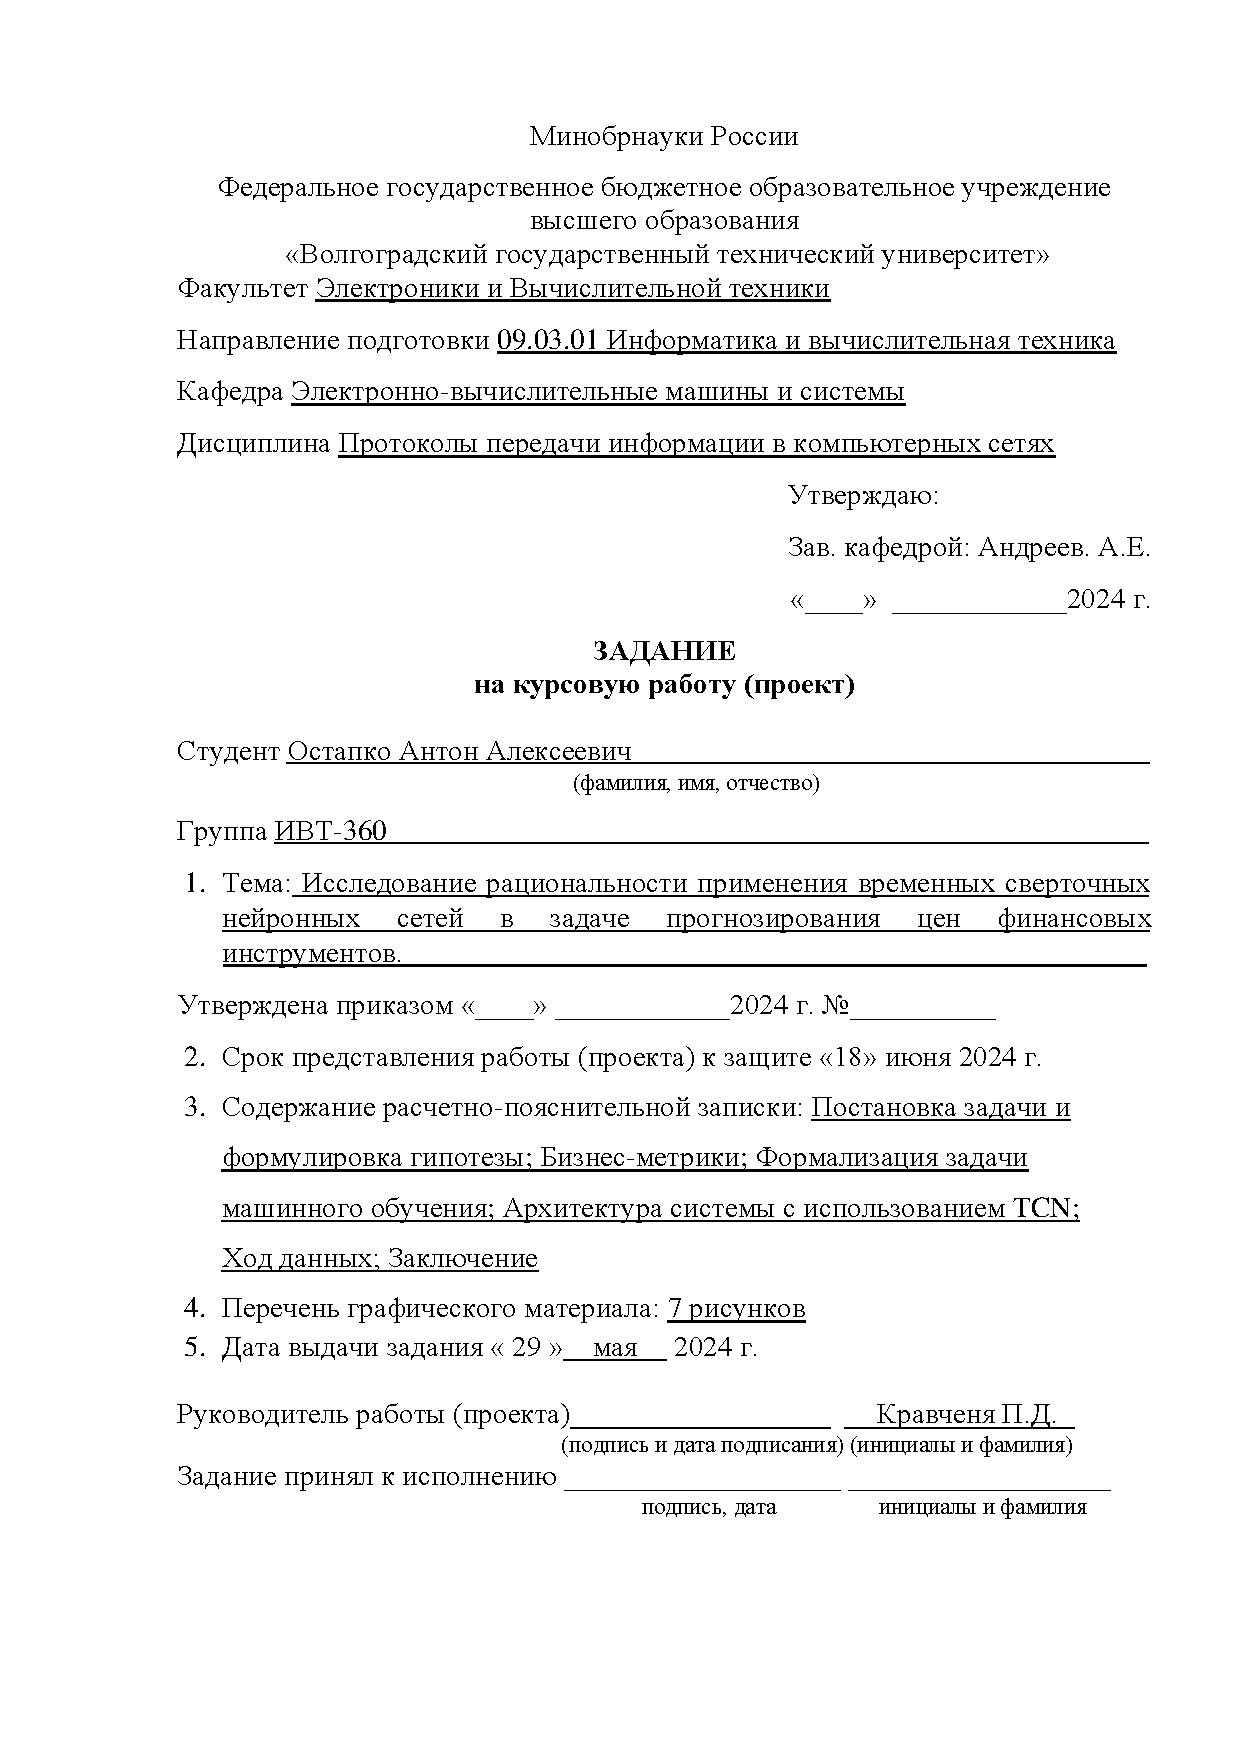
\includepdf[pages=-]{titlepage.pdf}

% Если нужно вставить свой титульный лист, то загрузите его в формате .pdf и переименуйте на titlepage, он вставится в начало документа
%%%%%%%%%%%%%%%%%%%%%%%%%%%%%%%%%%%%%%%%%%

%%%%%%%%%%%% Содержание %%%%%%%%%%%%%%%%%%
\newpage 
\begin{center}
    \tableofcontents
\end{center}
\newpage 
%%%%%%%%%%%%%%%%%%%%%%%%%%%%%%%%%%%%%%%%%%



%%%%%%%%%%%% Основной документ %%%%%%%%%%%%%%
\addcontentsline{toc}{section}{1 Постановка бизнес-задачи и формулировка гипотезы}

1 Постановка бизнес-задачи и формулировка гипотезы

Постановка бизнес-задачи

Задача заключается в разработке торговой стратегии для получения прибыли от операций с акциями Сбербанка (тикер: SBER), обращающимися на Московской Бирже. Основная цель – создание модели прогнозирования цен, которая сможет с высокой точностью предсказывать будущие изменения стоимости акций Сбербанка. Прогнозирование должно основываться на исторических данных о ценах, объемах торгов и других доступных метриках.
Для успешного выполнения задачи необходимо:

Сбор данных: Получить исторические котировки акций Сбербанка с сайта Finam. Данные должны включать цены открытия, закрытия, максимальные и минимальные цены за период, а также объемы торгов.

Предобработка данных: Очистить и нормализовать данные для улучшения качества модели. Это может включать удаление пропущенных значений, обработку выбросов и приведение данных к единому формату.

Разработка модели: Построить модель на основе временных сверточных нейронных сетей (Temporal Convolutional Networks, TCN). Для этого будет использован open-source проект keras-tcn.

Обучение модели: Обучить модель на исторических данных, используя различные комбинации гиперпараметров для достижения наилучших результатов.

Тестирование и валидация: Оценить качество модели на тестовом наборе данных, проведя валидацию с помощью метрик точности, таких как средняя абсолютная ошибка (MAE), среднеквадратичная ошибка (MSE) и другие.

Внедрение и адаптация: Разработать систему, которая будет использовать прогнозы модели для принятия торговых решений в реальном времени.


\newpage
Гипотеза

Гипотеза состоит в следующем: используя исторические данные о ценах и объемах торгов акциями Сбербанка, можно выявить скрытые паттерны и закономерности, которые помогут предсказать будущие изменения цены с достаточной точностью.

Основные аспекты гипотезы включают:

Существование паттернов: В исторических данных действительно присутствуют паттерны или закономерности, которые могут быть выявлены и использованы для прогнозирования. Например, комбинации цен открытия, закрытия, максимума, минимума и объемов торгов могут предсказывать будущие движения цены.

Эффективность TCN: Временные сверточные нейронные сети (TCN) способны эффективно обрабатывать временные ряды данных и выявлять сложные зависимости, которые не всегда очевидны при использовании традиционных методов анализа.

Прибыльность стратегии: Использование предсказаний модели для принятия торговых решений приведет к улучшению прибыльности торговых операций по сравнению с использованием случайных или традиционных методов анализа.
Для проверки гипотезы будут проведены следующие этапы:

Построение модели: Разработка и обучение TCN модели на исторических данных.

Анализ результатов: Оценка качества прогнозов на тестовых данных и сравнение с фактическими изменениями цен.

Таким образом, успешная реализация данной задачи поможет подтвердить или опровергнуть гипотезу о том, что временные сверточные нейронные сети могут быть эффективным инструментом для прогнозирования цен акций Сбербанка и разработки прибыльных торговых стратегий.
\newpage
\addcontentsline{toc}{section}{2 Бизнес-метрики}

2 Бизнес-метрики

Бизнес-метрики – это ключевые показатели, которые используются для оценки качества и эффективности различных бизнес-операций, в том числе и торговых стратегий. Они помогают количественно измерить успех или неудачу стратегий и позволяют проводить сравнительный анализ различных подходов. В контексте торговых стратегий, бизнес-метрики используются для оценки прибыльности, устойчивости и рисков, связанных с торговыми операциями. Эти метрики предоставляют объективные данные, которые необходимы для принятия обоснованных решений о покупке и продаже активов.

Для того, чтобы оценить качество торговой стратегии и её эффективности на рынке, в нашей работе необходимо проанализировать и использовать следующие бизнес-метрики:

Кумулятивная прибыль:


Кумулятивная прибыль представляет собой общую сумму прибыли, накопленную за весь период торговли.
Это ключевой показатель успешности стратегии, так как он демонстрирует общую результативность всех проведенных операций. Высокая кумулятивная прибыль указывает на эффективность стратегии в долгосрочной перспективе.

\[
\mathrm{Кумулятивная\ прибыль} = \sum_{i=1}^{N} P_i
\]
где \(P_i\) – прибыль от \(i\)-й сделки, \(N\) – общее количество сделок.

Максимальная просадка (Maximum Drawdown):

Максимальная просадка – это наибольшее падение стоимости портфеля от его максимального значения до минимального за определенный период времени.
Эта метрика показывает уровень риска стратегии, помогая понять, насколько сильно может снизиться стоимость портфеля в неблагоприятные периоды. Она критически важна для управления рисками и сохранения капитала.

\[
\mathrm{Максимальная\ Просадка} = \max_{t \in [0, T]} \left( \frac{\mathrm{Peak}_t - \mathrm{Trough}_t}{\mathrm{Peak}_t} \right),
\]
где \(\mathrm{Peak}_t\) – максимальная стоимость портфеля до падения, \(\mathit{Trough}_t\) – минимальная стоимость портфеля после пика.

Процент прибыльных сделок:

Процент прибыльных сделок – это доля сделок, которые завершились с прибылью, относительно общего числа сделок. Эта метрика позволяет оценить точность прогнозов и эффективность стратегии. Высокий процент прибыльных сделок указывает на высокую вероятность успешных прогнозов.

\[
\mathrm{Процент\ прибыльных\ сделок} = \left( \frac{N_{\text{прибыльных}}}{N_{\text{общих}}} \right) \times 100\%,
\]
где \(N_{\text{прибыльных}}\) – количество прибыльных сделок, \(N_{\text{общих}}\) – общее количество сделок.

Средняя прибыль/убыток на сделку:

Средняя прибыль/убыток на сделку – это средняя величина прибыли или убытка, полученная за одну сделку. Эта метрика помогает понять эффективность каждой отдельной сделки и оценить, насколько прибыльной является стратегия на уровне отдельных операций.

\[
\mathrm{Средняя\ прибыль/убыток\ на\ сделку} = \frac{\sum_{i=1}^{N} P_i}{N},
\]
где \(P_i\) – прибыль от \(i\)-й сделки, \(N\) – общее количество сделок.

Sharpe Ratio:

Sharpe Ratio демонстрирует соотношение средней доходности к стандартному отклонению доходности. Эта метрика позволяет оценить доходность торговой стратегии с учетом риска. Высокое значение Sharpe Ratio указывает на высокую доходность при относительно низком уровне риска, что является хорошим показателем.

\[
\mathrm{Sharpe\ Ratio} = \frac{R_p - R_f}{\sigma_p},
\]
где \(R_p\) – средняя доходность портфеля, \(R_f\) – безрисковая ставка доходности, \(\sigma_p\) – стандартное отклонение доходности портфеля.

Коэффициент выигрыш/проигрыш (Win/Loss Ratio):

Соотношение средней прибыли по выигрышным сделкам к средней потере по проигрышным сделкам. Высокий коэффициент говорит о высокой эффективности стратегии, показывая, что прибыльные сделки приносят больше дохода, чем убытки от убыточных сделок, то есть компенсируют потери от проигрышных, что является важным показателем эффективности стратегии.

\[
\mathrm{Win/Loss\ Ratio} = \frac{\mathrm{Средняя\ прибыль\ на\ выигрышную\ сделку}}{\mathrm{Средняя\ потеря\ на\ проигрышную\ сделку}},
\]

Частота сделок:

Количество сделок за определенный период (например, месяц или год). Эта метрика помогает понять активность стратегии и её потенциальные транзакционные издержки. Высокая частота сделок может указывать на активную торговлю, но может также повышать транзакционные издержки. Анализ частоты сделок помогает оптимизировать процесс торговли и управление рисками.

\[
\mathrm{Частота\ сделок} = \frac{N}{T},
\]
где \(N\) – общее количество сделок за период, \(T\) – длительность периода.

Каждая из этих метрик предоставляет важную информацию, которая помогает оценить эффективность и устойчивость разработанной торговой стратегии, позволяя выявить её сильные и слабые стороны, а также принять обоснованные решения для её оптимизации.

\newpage
\addcontentsline{toc}{section}{3 Формализация задачи машинного обучения}
3 Формализация задачи машинного обучения

Тип задачи:

Задача торговли акциями можно формализовать как задачу машинного обучения по предсказанию временных рядов (time series
forecasting) или задачу классификации для определения направления изменения цены.

Целевые переменные:

а) Для задачи регрессии (предсказание цены):

Целевая переменная: цена закрытия следующего дня (CLOSE следующего дня).

б) Для задачи классификации (предсказание направления):

Целевая переменная: бинарный показатель роста или падения цены на следующий день (например, 1 - цена повысится, 0 - цена
понизится).

Признаки (features):

Используем исторические данные для создания признаков:

а) Цена открытия (OPEN), закрытия (CLOSE), минимума (LOW), максимума (HIGH), объемы (VOL) за последние N дней.

б) Скользящие средние, разности между ценами (например, HIGH - LOW).

в) Технические индикаторы (SMA, EMA, RSI, MACD и др.).

г) Лагированные переменные (например, CLOSE предыдущего дня, OPEN предыдущего дня и т.д.).

Функция ошибки и метрики для ML:

а) Для задачи регрессии:

Функция ошибки: среднеквадратичная ошибка (\foreignlanguage{english}{Mean} \foreignlanguage{english}{Squared}
\foreignlanguage{english}{Error}, \foreignlanguage{english}{MSE}):
\[
\mathrm{MSE}=\frac 1 n\sum _{i=1}^n(y_i-\widehat
{y_i})^2
\]
где  $y_i$\ – истинные значения,  $\widehat {y_i}$\ – предсказанные значения.

Метрики \foreignlanguage{english}{ML}: среднеквадратичная ошибка (\foreignlanguage{english}{MSE}): как функция ошибки.

б) Для задачи классификации: логистическая функция потерь (\foreignlanguage{english}{Log} \foreignlanguage{english}{Loss}):
\[
 \log \mathrm{Loss}=\frac{-1} n\sum _{i=1}^n[y_i\log \left(\widehat {y_i}\right)+\left(1-y_i\right)\log(1-\widehat {y_i})]
 \]
 где  $y_i$\ – истинные метки,  $\widehat {y_i}$\ – предсказанные вероятности.

Функция ошибки: средняя абсолютная ошибка (\foreignlanguage{english}{Mean} \foreignlanguage{english}{Absolute}
\foreignlanguage{english}{Error}, \foreignlanguage{english}{MAE}):
\[
\mathrm{MAE}=\frac 1 n\sum _{i=1}^n\|
y_i-\widehat {y_i}\| 
\]
 где  $y_i$\ – истинные метки,  $\widehat {y_i}$\ – предсказанные вероятности.
 
Коэффициент детерминации $R^2$ является метрикой для оценки качества регрессионной модели. Он измеряет долю вариации зависимой переменной (целевой переменной) в данных, которая может быть объяснена моделью. Чем ближе значение $R^2$ к 1, тем лучше модель объясняет данные и тем выше её предсказательная способность.

Метрики ML:

Accuracy (точность) - это метрика для задач классификации, которая измеряет долю правильно классифицированных наблюдений среди всех наблюдений. Она выражает способность модели правильно идентифицировать все классы в общем числе примеров.

Precision и Recall:

Precision измеряет долю истинных положительных результатов среди всех предсказанных положительных результатов. Она подходит, когда важно минимизировать количество ложных положительных результатов.

Recall измеряет долю истинных положительных результатов среди всех истинных положительных результатов в данных. Она полезна, когда необходимо минимизировать количество ложных отрицательных результатов.

F1-Score представляет собой гармоническое среднее между Precision и Recall. Он дает общую оценку точности и полноты классификации. Высокое значение F1-Score указывает на хороший баланс между Precision и Recall.

ROC-AUC (площадь под ROC-кривой) является метрикой, используемой для измерения способности модели различать между классами. ROC-кривая представляет собой график, показывающий зависимость между долей ложных положительных результатов (FPR) и долей истинных положительных результатов (TPR) при изменении порогового значения классификации. Площадь под ROC-кривой (ROC-AUC) является числовым значением, отражающим общую способность модели различать между классами. Чем выше ROC-AUC, тем лучше модель различает классы.

Оптимизация бизнес-метрик через ML:

Регуляризация:

Регуляризация, такая как L1 или L2, применяется для предотвращения переобучения модели. Она добавляет штрафы за сложность модели, управляя весами признаков и улучшая её обобщающую способность. Это особенно важно в случае финансовых данных, где модели часто сталкиваются с переобучением из-за сложности временных зависимостей.

Гиперпараметрическая оптимизация:

Для настройки моделей на оптимальные значения гиперпараметров используются методы кросс-валидации, Grid Search, Random Search и Bayesian Optimization. Эти методы позволяют искать наилучшие параметры модели, что существенно повышает её эффективность и точность предсказаний на реальных данных.

Feature Engineering:

Создание новых признаков на основе технического анализа (например, скользящие средние, индикаторы MACD, RSI) и экспертных знаний в области финансов играет ключевую роль в улучшении качества моделей. Хорошо спроектированные признаки могут значительно улучшить способность модели к захвату временных зависимостей и предсказанию изменений цен.

Сложные модели:

Применение сложных алгоритмов, таких как Random Forest, Gradient Boosting, рекуррентные нейронные сети (RNN), LSTM, помогает захватить более сложные временные зависимости в данных. Эти модели способны автоматически извлекать и использовать скрытые паттерны, что особенно важно в анализе финансовых временных рядов.

Анализ ошибок:

Систематический анализ неправильных предсказаний помогает идентифицировать слабые стороны модели и направляет улучшения в алгоритмах. Это включает в себя идентификацию причин ошибок и корректировку алгоритмов для улучшения качества предсказаний.

Связь ML-метрик с бизнес-метриками

Высокие значения ML-метрик, таких как MSE, $R^2$, Log Loss, Precision, Recall и F1-Score, напрямую влияют на улучшение бизнес-метрик в торговых стратегиях. Например, точные предсказания цен (высокий $R^2$, низкий MSE) способствуют лучшему определению точек входа и выхода, что улучшает кумулятивную прибыль и снижает риски. Высокая точность и полнота классификации (Accuracy, Precision, Recall, F1-Score) помогают правильно идентифицировать моменты покупки и продажи, что также ведет к улучшению финансовых результатов и снижению максимальной просадки.


Таким образом, оптимизация моделей машинного обучения через указанные методы является критически важной для успешного применения торговых стратегий на финансовых рынках, обеспечивая высокую точность предсказаний.

Оптимизация ML-метрик, таких как MSE, $R^2$, Log Loss, Precision, Recall и F1-Score, напрямую повлияет на улучшение бизнес-метрик, таких как кумулятивная прибыль, максимальная просадка и коэффициент выигрыш/проигрыш.

\newpage
\addcontentsline{toc}{section}{4 Архитектура системы с использованием TCN}
4 Архитектура системы с использованием TCN

Общая архитектура системы:

Система для автоматизированной торговли акциями Сбербанка с использованием TCN включает следующие основные компоненты:

Компоненты системы

а) Сбор данных:

Исторические данные: данные о ценах и объемах торгов из различных источников, таких как файлы CSV и API.

Потоковые данные в реальном времени: данные, поступающие в систему непосредственно во время торгов, используя протоколы типа WebSockets или API.

б) Предобработка данных:

Очистка данных: удаление ошибок, аномалий и обработка пропущенных значений.

Создание признаков (feature engineering): формирование новых признаков на основе исторических данных, таких как скользящие средние, технические индикаторы (например, SMA, EMA, RSI, MACD) и лагированные переменные.

Нормализация и стандартизация данных: приведение данных к единому масштабу для обеспечения стабильности работы модели.

в) Модели прогнозирования:

TCN модель для прогнозирования цены/направления: использование Temporal Convolutional Networks для анализа временных рядов и предсказания цены закрытия следующего дня или направления изменения цены.

Модели для технического анализа: дополнительные модели или технические индикаторы для поддержки решений о торговле.

г) Система принятия решений:

Алгоритмы для генерации торговых сигналов: используются для определения точек входа и выхода на основе прогнозов модели TCN и других индикаторов.

Управление рисками и стратегиями: алгоритмы для контроля рисков и выбора оптимальных стратегий торговли.

д) Исполнение торговых операций:

Интерфейс с торговой платформой или брокером: программный интерфейс для автоматизации и исполнения торговых операций, основанный на сгенерированных торговых сигналах.

е) Мониторинг и управление:

Отслеживание производительности системы: мониторинг работы системы, времени отклика и других ключевых метрик.
Реагирование на сбои и аномалии: автоматическое оповещение и реагирование на непредвиденные события.
Обратная связь для адаптации и обучения модели: анализ результатов торговли для обновления модели и улучшения ее прогностической способности.

Место TCN модели в архитектуре:

а) Сбор данных

Компонент: Датчики и интерфейсы для сбора данных.

Задача: Получение исторических данных и потоковых данных в реальном времени.

б) Предобработка данных

Компонент: Сервис предобработки данных.

Задача: Очистка данных, создание новых признаков, нормализация данных для подачи в модель.

Инструменты\foreignlanguage{english}{: Pandas, NumPy, Scikit-learn.}

в) Модели прогнозирования

Компонент: Модуль TCN модели.

Задача: Прогнозирование цены закрытия на следующий день или направления изменения цены.

Место TCN модели:

Использование TCN для анализа временных рядов и захвата временных зависимостей.

Обучение модели на исторических данных и использование для прогнозов в реальном времени.

Инструменты: TensorFlow, Keras, PyTorch.

г) Система принятия решений

Компонент: Алгоритм генерации торговых сигналов.

Задача: Генерация торговых сигналов (покупка/продажа) на основе прогнозов TCN модели и других индикаторов.

Инструменты\foreignlanguage{english}{: Custom Logic, Scikit-learn, Pandas.}

д) Исполнение торговых операций

Компонент: Торговый бот.

Задача: Интерфейс с брокерской платформой для исполнения торговых сигналов.

Инструменты\foreignlanguage{english}{: API }брокера\foreignlanguage{english}{, Alpaca, Interactive Brokers.}

е) Мониторинг и управление

Компонент: Система мониторинга.

Задача: Отслеживание состояния системы, логирование и оповещения.

Инструменты\foreignlanguage{english}{: Prometheus, Grafana, ELK Stack.}

Детализация TCN модели:

Детализация TCN модели включает несколько ключевых аспектов, начиная от входного слоя до выходного слоя, что позволяет ей эффективно обрабатывать временные ряды и делать прогнозы как для задач регрессии, так и классификации.

Архитектура TCN модели

Входной слой:

На вход TCN модели поступают признаки за последние N дней, включая цены закрытия, объемы торгов и технические индикаторы. Эти признаки формируют входные данные, которые модель использует для анализа временных зависимостей.

Слои TCN:

TCN (Temporal Convolutional Network) включает в себя несколько последовательных слоев, специально разработанных для захвата временных зависимостей во временных рядах. Каждый слой TCN обычно содержит операции свертки и пулинга, что позволяет модели извлекать иерархические признаки из последовательности данных.

Полносвязный слой:

После последнего слоя TCN следует один или несколько полносвязных (Dense) слоев. Эти слои используются для обработки выходных данных от TCN, что позволяет модели агрегировать признаки и подготовить данные к финальному предсказанию.

Выходной слой:

На выходе TCN модели может быть настроен различный тип выходного слоя в зависимости от задачи:.

Для задачи регрессии: один нейрон на выходном слое, который выдает числовое предсказание цены на следующий день.

Для задачи классификации: один нейрон с сигмоидной активацией, который выдает вероятность роста цены. Это позволяет модели предсказывать вероятность изменения направления цены (например, вероятность того, что цена вырастет).

Архитектура TCN модели представляет собой эффективное сочетание слоев для анализа временных данных с последующими полносвязными слоями для обработки и вывода результатов. Такая структура позволяет модели точно предсказывать временные ряды и использовать полученные прогнозы для принятия решений в автоматизированной торговле.

\newpage
\addcontentsline{toc}{section}{5 Ход работы}
5 Ход работы

Импорт библиотек и начальные настройки:

\begin{minted}
{text}
import glob
import numpy as np
import pandas as pd
import plotly.express as px
import seaborn as sns
import tensorflow as tf
from sklearn.model_selection import train_test_split
from sklearn.preprocessing import OneHotEncoder, RobustScaler, StandardScaler
from sklearn.impute import SimpleImputer

%load_ext tensorboard
print("Num GPUs Available: ", len(tf.config.list_physical_devices('GPU')))
\end{minted}

В этом блоке кода мы импортируем необходимые библиотеки для анализа данных, визуализации и машинного обучения. Среди них:

glob: для работы с файловыми путями.

numpy и pandas: для работы с данными.

plotly.express и seaborn: для визуализации данных.

tensorflow: для создания и обучения моделей нейронных сетей.

sklearn: для предобработки данных и разбиения их на обучающие и тестовые наборы.

Затем загружаем расширение tensorboard для мониторинга процесса обучения модели и проверяем наличие доступных GPU.

Загружаем датасет из CSV-файла в DataFrame с помощью библиотеки pandas и выводим первые пять строк для ознакомления с данными:

\begin{minted}
{text}
df = pd.read_csv('SBER.csv',encoding='cp1251')
print(df.head(5))
\end{minted}

\image{Screenshot_1.png}{}{1}{Рисунок 1 – Результат предпросмотра данных}

Этот код выводит первые пять строк датафрейма. Комментарии к столбцам:

TICKER: Наименование инструмента.

PER: Период.

DATE: Дата.

TIME: Время.

OPEN: Цена открытия свечи (только бары).

LOW: Цена минимума свечи (только бары).

HIGH: Цена максимума свечи (только бары).

CLOSE: Цена закрытия свечи (только бары).

VOL: Объем бара (или сделки).

Посмотрим как выглядит датасет:

\image{Screenshot_2.png}{}{0.82}{Рисунок 2 – Вид датасета}


Выводим информацию о датасете, включая количество записей и типы данных в каждом столбце:
\image{Screenshot_3.png}{}{0.7}{Рисунок 3 – Информация о датасете}

Устанавливаем библиотеку keras-tcn, необходимую для использования временных сверточных сетей (TCN):

\begin{minted}
{text}
!pip install keras-tcn
\end{minted}

Нормализация данных:

Используем StandardScaler для нормализации данных, чтобы привести их к единому масштабу, что необходимо для корректной работы моделей машинного обучения.

\begin{minted}
{text}
from sklearn.preprocessing import StandardScaler

scaler = StandardScaler()
df_scaled = scaler.fit_transform(df[['OPEN', 'HIGH', 'LOW', 'CLOSE', 'VOL']])
\end{minted}

Подготовка данных для модели:

Подготавливаем входные данные и целевую переменную для модели. Используем последние N дней для предсказания следующего значения.

\begin{minted}
{text}
X = []
y = []
N = 10  # количество дней для TCN
for i in range(N, len(df_scaled)):
    X.append(df_scaled[i-N:i])
    y.append(df['TARGET'].iloc[i])
X = np.array(X)
y = np.array(y)
\end{minted}

Разделяем данные на обучающую и тестовую выборки в соотношении 80/20.

\begin{minted}
{text}
X_train, X_test, y_train, y_test = train_test_split(X, y, test_size=0.2,
random_state=42)
\end{minted}

Создаем модель с использованием временных сверточных сетей (TCN) для анализа временных рядов и предсказания значения.

\begin{minted}
{text}
def build_tcn_model(input_shape):
    model = Sequential([
        TCN(input_shape=input_shape),
        Dense(1)  # Для регрессии
    ])
    model.compile(optimizer='adam', loss='mse', metrics=['mae'])
    return model

input_shape = (N, X_train.shape[2])
model = build_tcn_model(input_shape)
\end{minted}

Обучаем модель на обучающих данных и валидируем на тестовых данных в течение 1000 эпох. Наблюдаем за тем, как меняются значения с каждой эпохой.

\begin{minted}
{text}
history = model.fit(X_train, y_train, epochs=1000, validation_data=(X_test,
y_test), batch_size=32)
\end{minted}

\image{Screenshot_6.png}{}{1}{Рисунок 4 – Результат последних эпох}

Оцениваем модель на тестовых данных, выводим метрику MAE (Mean Absolute Error).

\begin{minted}
{text}
loss, mae = model.evaluate(X_test, y_test)
print(f'Test MAE: {mae}')
\end{minted}

Делаем предсказания на тестовых данных и вычисляем дополнительные метрики MSE (Mean Squared Error) и $R^2$ (коэффициент детерминации).

\begin{minted}
{text}
y_pred = model.predict(X_test)
from sklearn.metrics import mean_squared_error, r2_score

mse = mean_squared_error(y_test, y_pred)
r2 = r2_score(y_test, y_pred)

print(f'Test MSE: {mse}')
print(f'Test R^2: {r2}')
\end{minted}

\image{Screenshot_4.png}{}{1}{Рисунок 5 – Оценка модели}

Строим график для визуального сравнения фактических и предсказанных значений.

\begin{minted}
{text}
import matplotlib.pyplot as plt
plt.figure(figsize=(14, 7))
plt.plot(y_test, label='Actual Values')
plt.plot(y_pred, label='Predicted Values')
plt.xlabel('Sample')
plt.ylabel('Closing Price')
plt.title('Actual vs Predicted Closing Prices')
plt.legend()
plt.show()
\end{minted}

\image{Screenshot_5.png}{}{1}{Рисунок 6 – Визуализация результатов}

Выводим первые десять фактических и предсказанных значений для проверки качества предсказаний модели.

\begin{minted}
{text}
for i in range(10):
    print(f'Actual: {y_test[i]:.2f}, Predicted: {y_pred[i][0]:.2f}')
\end{minted}

\image{Screenshot_7.png}{}{0.6}{Рисунок 7 – Вывод предсказанных и фактических значений}

\addcontentsline{toc}{section}{Заключение}
Заключение

Метрики производительности:

Mean Absolute Error (MAE): Полученное значение MAE составляет 32.45, что указывает на среднее отклонение предсказанных значений от фактических.

Mean Squared Error (MSE): Значение MSE составляет 1530.40, отражая среднеквадратичную ошибку предсказаний модели.

R²: Несмотря на отрицательное значение (-0.88), указывающее на то, что модель может быть лучше, чем простая средняя величина, результаты говорят о том, что модель нуждается в доработке для лучшего объяснения вариации данных.

Визуализация результатов: График фактических и предсказанных значений показал наличие расхождений между предсказанными и реальными значениями цен закрытия. 

Работа показала потенциал модели TCN в предсказании цен закрытия акций, однако требует дальнейших улучшений для достижения более точных результатов. 
%%%%%%%%%%%%%%%%%%%%%%%%%%%%%%%%%%%%%%%%%%


\end{document}


%%%%%%%%%%%%%%%%%%%%%%%%%%%%%%%%%%%%%%%%%%